Pour être plus clair, nous avons voulu séparer chaque module dans un dossier différent.
Pour cela il faut créer un fichier \lstinline{<nom-module>.gpr} dans le dossier définissant le module : 
\begin{lstlisting}[language=Ada, caption={Fichier générique *.gpr définissant un nouveau module}, label={nouveau-module}]
   project Nom_Module is
       for Source_Dirs use (".");
       for Object_Dir use "../obj";
   end Nom_Module;
\end{lstlisting}

Pour pouvoir se servir d'un module \lstinline{A} dans un module \lstinline{B} il faut importer le module \lstinline{A} dans le fichier \lstinline{module-b.gpr} : 
\begin{lstlisting}[language=Ada, caption={Import de module}]
   with "<chemin-relatif-du-module>/<nom-du-module>";
   ...
\end{lstlisting}

La Figure \ref*{fig : structure_fichiers_projet} représente la structure des fichiers de notre projet. On peut remaquer qu'il y a un dossier \lstinline{obj}. Lors de la compilation, le compilateur génère une multitude de fichiers... Pour éviter qu'ils ne polluent nos dossiers, on a dit à chaque module de générer ses fichiers de compilation dans un seul dossier (ligne 3 du Code \ref*{nouveau-module})

\begin{figure}[ht!]
   \centering
   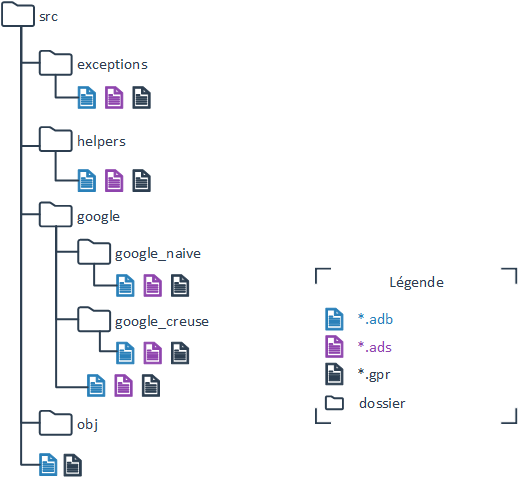
\includegraphics[scale=0.8]{partie-2/sous-partie-2/structure_fichier.png}
   \caption{Structure des fichiers \label{fig : structure_fichiers_projet}}
\end{figure}

